% DS-PIT architecture --- v4.1 (2026-09-22).
% v4：对齐版本（六框等高、列中心统一、组框同宽、回环为直线）。
% v4.1：按 nature-figure 审计修正字号地板 —— 原 \scriptsize 正文在 PDF 中
%       渲染为 4.98 pt（低于 5 pt 下限），改为 \footnotesize（正文）与
%       \small（小标题），并按放大后的字号重排画布（框宽 84 pt、列距 94 pt）。
% 回环：温度经左侧竖线回似然（红虚线），发射值经右侧竖线回缓冲（蓝虚线）。
% Compile: pdflatex DS-PIT_chart2_v4.tex  ->  DS-PIT_chart2_v4.pdf
\documentclass[border=3pt]{standalone}
\usepackage{tikz}
\usepackage{amsmath,amssymb}
\usetikzlibrary{arrows.meta, positioning, calc}

\definecolor{blkblue}{HTML}{E9EEF8}
\definecolor{blkblueb}{HTML}{3C63A0}
\definecolor{blkcream}{HTML}{FAF2E2}
\definecolor{blkcreamb}{HTML}{A9762F}
\definecolor{blkgreen}{HTML}{E8F4E9}
\definecolor{blkgreenb}{HTML}{3B7442}
\definecolor{blkred}{HTML}{A93B2B}
\definecolor{blkgray}{HTML}{3E3E3E}

\newcommand{\hd}{\small\bfseries}
\newcommand{\tx}{\footnotesize}

\begin{document}
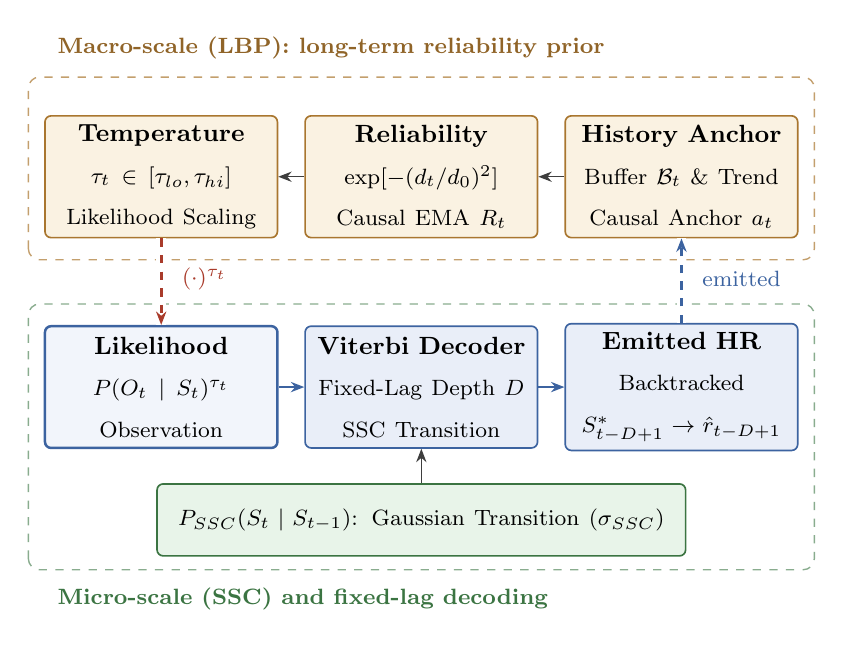
\begin{tikzpicture}[x=1pt, y=1pt,
  >={Stealth[length=1.7mm,width=1.3mm]},
  arr/.style={->, draw=blkgray, line width=0.5pt},
  fwd/.style={->, draw=blkblueb, line width=1pt},
  tpath/.style={->, draw=blkred, line width=1pt, dashed},
  halo/.style={white, line width=3.4pt},
  base/.style={draw, rounded corners=2.2pt, align=center, inner sep=3pt,
               line width=0.6pt, text width=78pt, minimum height=44pt},
  mac/.style={base, fill=blkcream, draw=blkcreamb},
  dec/.style={base, fill=blkblue, draw=blkblueb},
  obs/.style={base, fill=blkblue!60, draw=blkblueb, line width=0.9pt},
  hd/.style={font=\small\bfseries},
  tx/.style={font=\footnotesize},
  lab/.style={font=\footnotesize}
]

% ---- group frames: same width, same left inset, title strip outside ------
\draw[draw=blkcreamb!70, dashed, rounded corners=4pt, line width=0.5pt]
      (8,120) rectangle (292,186);
\draw[draw=blkgreenb!60, dashed, rounded corners=4pt, line width=0.5pt]
      (8,8) rectangle (292,104);
\node[font=\footnotesize\bfseries, text=blkcreamb!85!black, anchor=south west]
      at (15,189) {Macro-scale (LBP): long-term reliability prior};
\node[font=\footnotesize\bfseries, text=blkgreenb, anchor=north west]
      at (15,5) {Micro-scale (SSC) and fixed-lag decoding};

% ---- macro-scale row (right -> left), centre y = 150 ---------------------
\node[mac] (tau) at (56,150)
      {{\hd Temperature}\\[3pt]{\tx $\tau_t \in [\tau_{lo},\tau_{hi}]$}\\[3pt]{\tx Likelihood Scaling}};
\node[mac] (rel) at (150,150)
      {{\hd Reliability}\\[3pt]{\tx $\exp[-(d_t/d_0)^2]$}\\[3pt]{\tx Causal EMA $R_t$}};
\node[mac] (buf) at (244,150)
      {{\hd History Anchor}\\[3pt]{\tx Buffer $\mathcal{B}_t$ \& Trend}\\[3pt]{\tx Causal Anchor $a_t$}};
\draw[arr] (buf.west) -- (rel.east);
\draw[arr] (rel.west) -- (tau.east);

% ---- decoder row (left -> right), centre y = 74 -------------------------
\node[obs] (o) at (56,74)
      {{\hd Likelihood}\\[3pt]{\tx $P(O_t\mid S_t)^{\tau_t}$}\\[3pt]{\tx Observation}};
\node[dec] (v) at (150,74)
      {{\hd Viterbi Decoder}\\[3pt]{\tx Fixed-Lag Depth $D$}\\[3pt]{\tx SSC Transition}};
\node[dec] (e) at (244,74)
      {{\hd Emitted HR}\\[3pt]{\tx Backtracked}\\[3pt]{\tx $S_{t-D+1}^* \to \hat r_{t-D+1}$}};
\draw[fwd] (o.east) -- (v.west);
\draw[fwd] (v.east) -- (e.west);

% ---- micro-scale box (centred under the decoder) -------------------------
\node[base, fill=blkgreen, draw=blkgreenb, text width=185pt, minimum height=26pt]
      (ssc) at (150,26)
      {{\tx $P_{SSC}(S_t\mid S_{t-1})$: Gaussian Transition ($\sigma_{SSC}$)}};
\draw[arr] (ssc.north) -- (v.south);

% ---- closed loop: temperature -> likelihood, emitted HR -> anchor --------
\draw[halo] (tau.south) -- (o.north);
\draw[tpath] (tau.south) -- (o.north);
\node[lab, text=blkred, anchor=west] at (60,113) {$(\cdot)^{\tau_t}$};

\draw[halo] (e.north) -- (buf.south);
\draw[fwd, dashed] (e.north) -- (buf.south);
\node[lab, text=blkblueb, anchor=west] at (248,113) {emitted};

\end{tikzpicture}
\end{document}
